%%%%%%%%%%%%%%%%%%%%%%%%%%%%%%%%%%%%%%%%%%%
%
% szablon pracy licencjackiej 
% korzystający ze stylu pracalicmgr.cls
% 2017.03.22 K. Turzynski
% 2017.03.01 P. Durka durka@fuw.edu.pl 
% na podstawie pliku J. Żygierewicz 2016
%
%%%%%%%%%%%%%%%%%%%%%%%%%%%%%%%%%%%%%%%%%%%



\documentclass{pracalicmgr}
\usepackage{polski}
\usepackage[utf8]{inputenc}
\usepackage{float}
\usepackage{booktabs}
\usepackage{hyperref}
\usepackage{url}
\usepackage{caption}
\usepackage{subcaption}
\usepackage{graphicx}
\usepackage[backend=bibtex]{biblatex}

\addbibresource{bibliografia.bib}

\author{Agnieszka Ciepielewska}

\nralbumu{385537}

\title{Zastosowanie uczenia maszynowego do identyfikacji leptonów tau w eksperymencie CMS}

\tytulang{Application of machine learning to identify tau leptons in the CMS experiment}

\kierunek{Fizyka w ramach Międzywydziałowych Indywidualnych
Studiów Matematyczno-Przyrodniczych}

% \specjalnosc{}

\opiekun{dr hab. Artur Kalinowski \\ Zakład Cząstek i Oddziaływań Fundamentalnych \\ Instytut Fizyki Doświadczalnej}

%\dziedzina{13.200}
\dziedzina{13.2 Fizyka}

\date{$<$TODO: miesiąc-i-rok-złożenia-pracy$>$}

\keywords{$<$TODO: wykaz maksymalnie 10 słów swobodnie wybranych$>$}



\begin{document}


    \maketitle
    \let\cleardoublepage\clearpage
    
    \begin{abstract}
    %TODO
$<$Krótkie (maks. 800 znaków) streszczenie pracy, na przykład:

Lorem ipsum – tekst składający się z łacińskich i quasi-łacińskich wyrazów, mający korzenie w klasycznej łacinie, wzorowany na fragmencie traktatu Cycerona „O granicach dobra i zła” (De finibus bonorum et malorum) napisanego w 45 r. p.n.e. Tekst jest stosowany do demonstracji krojów pisma (czcionek, fontów), kompozycji kolumny itp. Po raz pierwszy został użyty przez nieznanego drukarza w XVI w.

Tekst w obcym języku pozwala skoncentrować uwagę na wizualnych aspektach tekstu, a nie jego znaczeniu.

Cytat z {\tt https://pl.wikipedia.org/wiki/Lorem\_ipsum}
$>$

    \end{abstract}

    \tableofcontents
    
    \chapter*{Cel pracy}
    \addcontentsline{toc}{chapter}{Cel pracy}
    %TODO
    \chapter{Wstęp}
    \label{ch:wstep}
	%TODO    
    Tutaj piszemy informacje wprowadzające w tematykę  pracy, potrzebne do zrozumienia treści.       
    \section{Leptony tau}
    
    Leptony tau	odgrywają istotną rolę w wielu eksperymentach fizycznych. Jednym z ważniejszych jest badanie bozonu Higgs'a dzięki rozpadowi $H \rightarrow \tau\tau$. Jednak z powodu krótkiego czasu życia $T_{1/2} = 2.9 \cdot 10^{-13}~\mathrm{s}$ \cite{particle_physics}, one również nie są wykrywane bezpośrednio w eksperymentach, ale obserwuje się ich produkty rozpadu. Taony są najcięższymi z leptonów i przy swojej masie $m_\tau = 1.776 ~\mathrm{GeV}$ \cite{particle_physics} jako jedyne są w stanie rozpadać się hadronowo. Z tabeli \ref{tab:kanaly_rozpadu} widać, że dzieje się tak w około $2/3$ przypadków. Sprawia to problemy przy ich identyfikacji, ponieważ łatwo jest je pomylić z jetami hadronowymi (\textit{QCD jets}).
    
	\begin{table}[H]
	\centering
	\begin{tabular}{lr}
	\toprule
	Rozpad & Prawdopodobieństwo [\%] \\
	\midrule
	\multicolumn{2}{c}{Rozpady leptonowe} \\
	\midrule
	$\tau^- \rightarrow e^-\bar{\nu}_{e}\nu_{\tau}$ & $17.8$ \\
	$\tau^- \rightarrow \mu^-\bar{\nu}_{\mu}\nu_{\tau}$ & $17.4$ \\
	\midrule
	\multicolumn{2}{c}{Rozpady hadronowe} \\
	\midrule
	$\tau^- \rightarrow h^- \pi^0 \nu_{\tau}$ & $25.9$ \\
	$\tau^- \rightarrow h^-\nu_{\tau}$ & $11.5$ \\
	$\tau^- \rightarrow h^- h^+ h^- \nu_{\tau}$ & $9.8$ \\
	$\tau^- \rightarrow h^- \pi^0 \pi^0 \nu_{\tau}$ & $9.5$ \\
	$\tau^- \rightarrow h^- h^+ h^- \pi^0 \nu_{\tau}$ & $4.8$ \\
	Inne & $3.3$ \\	
	\bottomrule
	\end{tabular}
	\caption{Główne kanały rozpadu taonów wraz z prawdopodobieństwem \cite{tauid13, particle_physics}. Tutaj $h$ oznacza zarówno mezony $\pi$ jak i $K$.}
	\label{tab:kanaly_rozpadu}
	\end{table}
        
    \section{Detektor CMS}
	Detektor CMS (\textit{Compact Muon Solenoid}) znajduje się w Wielkim Zderzaczu Hadronów (LHC) w CERN-ie. Tam dokonywany jest eksperyment, z którego dane są wykorzystywane do rozpoznawania leptonów tau. Jego główne elementy to: nadprzewodząca cewka wytwarzająca pole magnetyczne o indukcji 3.8 T, detektory krzemowe, kalorymetr elektromagnetyczny (ECAL), kalorymetr hadronowy (HCAL) i komora jonizacyjna do wykrywania mionów. 
	
	Detektor krzemowy, pokrywający przedział pseudopospieszności $|\eta| < 2.5$, składa się z dwóch rodzajów detektorów: typu \textit{pixel} i typu \textit{strip}. Korpus centralny składa się z trzech warstw detektorów \textit{pixel} oraz jedenastu warstw detektorów \textit{strip}, natomiast końcówki z jedenastu dysków, z czego dwa zawierają detektory \textit{pixel}, a pozostałe detektory \textit{strip} \cite{cms_technical}. Tor lotu hadronów jest rekonstruowany ze skutecznością 80-90\% w zależności od pędu poprzecznego i pseudopospieszności $\eta$. Detektory krzemowe mają grubość od 0.4 do 2.0 długości drogi radiacyjnej ($X_0$), także fotony z dużym prawdopodobieństwem rozpadają się wewnątrz detektora na pary $e^+e^-$ \cite{tauid13}.
	
	Kalorymetr ECAL jest zrobiony ze scyntylacyjnych kryształów stolzytu (PbWO$_4$). Posiada ponad 61000 kryształów w korpusie centralnym, pokrywającym $|\eta| < 1.48$ oraz ponad 7300 kryształów na końcach detektora, pokrywających $|\eta| < 3.0$. Stolzyt posiada krótką drogę radiacyjną ($X_0 = 0.89$ cm), krótki promień Molièra (2.2 cm) oraz szybko wyświeca światło (80\% światła jest wyświecane w 25 ns). Dzięki temu dobrze rozdziela kaskady, więc jest często wykorzystywany do budowy kalorymetrów \cite{cms_technical}.
	
	Na zewnątrz ECAL znajduje się kalorymetr hadronowy HCAL zawierający mosiądz i plastik. Mosiądz został wybrany ze względu na krótką drogę swobodną (\textit{interaction length}) hadronów oraz słabe właściwości magnetyczne. %TODO nie pamiętam jak jest interaction length po polsku...
Tak samo jak ECAL pokrywa obszar $|\eta| < 3.0$. Jego grubość to od siedmiu do jedenastu dróg swobodnych w zależności od $\eta$. Natomiast dla $3.0 < \eta < 5.0$ używany jest stalowo kwarcowy kalorymetr \textit{Hadron Forward} \cite{cms_technical}.
	
	
	Detektor mionowy składa się z trzech rodzajów komór gazowych. W części centralnej ($|\eta| < 1.2$) używane są komory \textit{drift tube} (DT), w części końcowej ($|\eta| < 2.4$), pole magnetyczne nadal jest duże, ale niejednolite, używa się \textit{cathode strip chambers} (CSC). Dodatkowo we wszystkich miejscach są zastosowane \textit{resistive plate chambers} (RPC). RPC zapewnia dobrą dokładność czasową, natomiast DT i CSC dobrą dokładność pozycyjną \cite{cms_technical}.
	
	\section{Sieci neuronowe}
	Sieci neuronowe to klasa modeli uczenia maszynowego stosowana w uczeniu nadzorowanym. Na podstawie danych treningowych zawierający zmienne objaśniające i objaśniane model uczy się zależności występujących między tymi zmiennymi. Dzieki temu możliwe jest stosowanie modelu do predykcji zmiennych objaśnianych na podstawie nowych obserwacji.
	
	Sieci neuronowe składają się z warstw. Podstawową warstwą używaną w sieciach neuronowych jest warstwa gęsta (\textit{dense layer} lub \textit{fully connected layer}). Warstwa gęsta przyjmuje na wejściu wektor, a na wyjściu zwraca wektor ustalonej wielkości, niekoniecznie tego samego rozmiaru. Jest to warstwa bardzo generyczna, jednak jej minusem jest duża liczba parametrów (sieć długo się trenuje, zajmuje dużo miejsca i może gorzej generalizować \cite{dl}). Każda warstwa gęsta składa się z dwóch podstawowych elementów: regresji liniowej oraz funkcji nieliniowej, zwanej funkcją aktywacji. Każda regresja liniowa posiada wagi $w_i$ oraz przesunięcia $b_i$ (\textit{bias}). Wyjście z warstwy definiowane jest jako: $$y = f(x^TW + b),$$ gdzie $x$ to wektor wejściowy, $f$ - funkcja aktywacji, nie zmieniająca wymiaru wektora, $W$ - macierz wag warstwy, $b$ - wektor przesunięcia. 
	
	Dodanie kolejnych warstw to złożenie kolejnych takich funkcji.
	
	 Przykładowo na rysunku \ref{fig:simple} widoczne jest wejście do sieci $x$, które jest wektorem 3-elementowym. Następnie jest on transponowany i przemnażany przez macierz wag $W_1$, która jest wymiaru $3\times4$ oraz dodane jest przesunięcie $b_1$ o wymiarze $1\times4$. Na tym etapie nakłada się również funkcję aktywacji $f_1$. Kółka w warstwie ukrytej reprezentują wyjścia regresji liniowych już po zastosowaniu funkcji aktywacji. Kolejny krok jest analogiczny, tym razem jest to jedna regresja liniowa, czyli macierz wag $W_2$ ma wymiar $4\times1$, a przesunięcie $b_2$ $1\times1$. Zatem wyjście~$y$: $$y = f_2(f_1(x^TW_1 + b_1)W_2 + b_2),$$ gdzie $f_1, f_2$ to funkcje aktywacji. Zauważmy, że nieliniowe funkcje aktywacji są konieczne, gdyż inaczej wielowarstwową sieć neuronową zawsze dałoby się sprowadzić do przypadku zwykłej regresji liniowej odpowiednio przemnażając wagi \cite{dl}.
	
	\begin{figure}[H]
	\centering
	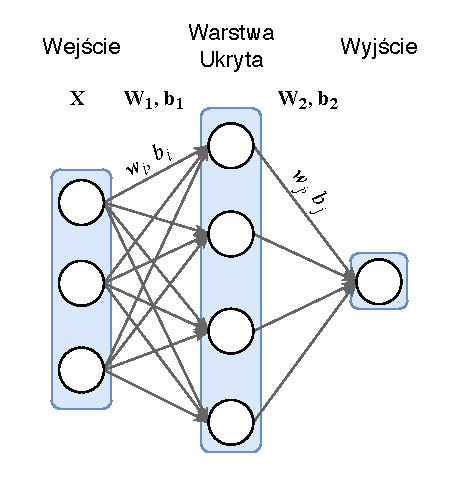
\includegraphics[width=0.5\textwidth]{simple_nn.pdf}
	\caption{Przykładowa sieć neuronowa z jedną ukrytą warstwą gęstą}
	\label{fig:simple}
	\end{figure}
	
	Następnie aby otrzymać optymalny model poszukiwane jest minimum funkcji straty (czyli miejsce, gdzie model najmniej się myli). Przez funkcję straty rozumiana jest funkcja przybliżająca błąd popełniany przez model. Nie da się wyznaczyć gradientu $L$ w każdym miejscu, ale można go znaleźć w punkcie, gdzie dokonywana jest predykcja. Także, aby poprawić wagi oraz przesunięcie w modelu używa się iteracyjnego algorytmu \textit{Gradient Descent}, który polega na obliczeniu gradientu funkcji straty po parametrach modelu $\nabla_{w_i}L$, a następnie aktualizowane są wagi o pewien krok w kierunku ujemnego gradientu, także dla przykładowej wagi $w$ przy $n+1$-szej iteracji (górny indeks oznacza numer iteracji): $$w^{(n+1)} \leftarrow w^{(n)} - \gamma \frac{\partial L^{(n)}}{\partial w^{(n)}},$$ gdzie $\gamma$ to tzw. stała uczenia (\textit{learning rate}) \cite{dl}. Widać, że istotne jest aby wszystkie funkcje użyte w modelu były różniczkowalne prawie wszędzie (w punktach nieciągłości pochodnej można przyjąć dowolną wartość brzegową). 

	
	\subsection{Funkcje aktywacji}
	Stosowane później funkcje aktywacji wraz ze wzorami:
	\begin{itemize}
	\item Sigmoid: $$S(x) = \frac{1}{1+e^{-x}},$$
	\item ReLU\cite{relu} $$ReLU(x) = \max(0, x).$$
	\end{itemize}
	
	\subsection{Warstwa \textit{batch normalization}}
	Sieci są uczone algorytmem \textit{Gradient Descent}, jednak aktualizacja wag sieci jest zazwyczaj wykonywana nie co jedną obserwację, a co pewną liczbę obserwacji (zwaną później \textit{batchem}). Taki algorytm nosi nazwę \textit{Stochastic Gradient Descent} (SGD). 
	
	Wraz z uczeniem sieci warstwy mogą zwracać inne wyjścia. W szczególności rozkład wyjścia może się zmieniać, do czego każda następna warstwa sieci musi się na nowo dostosowywać. Przeciwdziała temu warstwa \textit{batch normalization}, która przeskalowuje każdy batch tak aby miał tą samą średnią i odchylenie standardowe \cite{batch_norm}. Dzięki zastosowaniu \textit{batch normalization} trening sieci trwa krócej, a sieć może osiągnąć lepszą skuteczność.
	
	\subsection{Optymalizacja \textit{Adam}}
	Algorytm SGD często okazuje się niewystarczający, aby otrzymać dobre rezultaty. Dlatego często stosuje się algorytm \textit{Adam} (\textit{Adaptive momentum}) \cite{adam}.
	
	Zamiast zwykłego SGD, algorytm \textit{Adam} wyznacza aktualizację wag modelu na podstawie aktualnego oraz poprzednich gradientów. Liczy statystyki $m$, $v$ oraz ostateczną zmianę wag w następujący sposób \cite{adam}:
	$${\displaystyle m_{w}^{(n+1)}\leftarrow \beta _{1}m_{w}^{(n)}+(1-\beta _{1})\nabla _{w}L^{(n)}}$$$$
{\displaystyle v_{w}^{(n+1)}\leftarrow \beta _{2}v_{w}^{(n)}+(1-\beta _{2})(\nabla _{w}L^{(n)})^{2}} $$$$
{\displaystyle {\hat {m}}_{w}={\frac {m_{w}^{(n+1)}}{1-(\beta _{1})^{t+1}}}}$$$$ {\displaystyle {\hat {v}}_{w}={\frac {v_{w}^{(n+1)}}{1-(\beta _{2})^{t+1}}}}$$$$
{\displaystyle w^{(n+1)}\leftarrow w^{(n)}-\gamma {\frac {{\hat {m}}_{w}}{{\sqrt {{\hat {v}}_{w}}}+\epsilon }}}$$ gdzie $\beta_1, \beta_2$ to parametry, a $\epsilon$ to epsilon numeryczny.
	
	\subsection{TODO: callback}
	
	\subsection{Miary skuteczności modeli}
	Jako, że identyfikacja taonów to problem klasyfikacji binarnej, dobrą metryką do mierzenia skuteczności modelu jest ROC AUC (\textit{Area Under Receiver Operating Characteristic Curve}) oraz sama krzywa ROC. Analizowany model przewiduje prawdopodobieństwo, czy dany rozpad zawiera taon. Aby dokonać klasyfikacji musimy ustalić próg odcięcia ponad którym zawsze zwracane jest 1 (wystąpił taon), a poniżej 0 (nie wystąpił). Wówczas można policzyć \textit{true positive rate} (TPR) oraz \textit{false positive rate} (FPR). Krzywa ROC to wykres TPR od FPR dla różnych progów odcięcie.
	
	ROC AUC to pole pod krzywą ROC. W związku z tym przyjmuje ona wartości pomiędzy 0 a 1, gdzie 0.5 to wartość osiągana przez model losowy, zaś 1 przez bezbłędny klasyfikator. ROC AUC nie jest różniczkowalna, więc nie można jej bezpośrednio wykorzystać przy treningu sieci neuronowej jako funkcji straty. Jest jednak jest przydatna przy ewaluacji oraz porównywaniu wytrenowanych modeli.
	
	Do treningu wykorzystuje się zazwyczaj binarną entropię krzyżową (\textit{binary cross entropy}) \cite{dl}, daną wzorem: $$ L(y, p) = -(y\log(p)+(1-y)\log(1-p)),$$ gdzie $y$ to prawdziwe wartości, a $p$ to predykcje modelu.
	
	\section{XGBoost}
	XGBoost (\textit{eXtreme Gradient Boosting}) \cite{xgboost} to implementacja algorytmu \textit{Gradient Boosting}, polegającym na budowaniu kolejnych drzew decyzyjnych (rys. \ref{fig:tree}). Każde kolejne drzewo jest tworzone aby jak najlepiej przewidywać błąd popełniany przez poprzedni zestaw drzew. Końcowa predykcja to suma wszystkich odpowiedzi drzew.
	
	\begin{figure}[h]
	\centering
	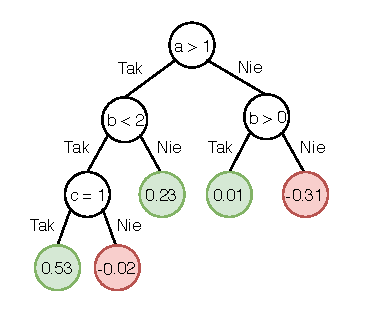
\includegraphics[width=0.5\textwidth]{tree.pdf}
	\caption{Przykładowe drzewo decyzyjne, $a, b, c$ to zmienne występujące w danych}
	\label{fig:tree}
	\end{figure}
	
    \chapter{Dane eksperymentalne oraz symulacyjne}
    \label{ch:dane}
    Dane eksperymentalne pochodzą ze zderzeń pp z eksperymentu CMS. %TODO energia i rok?
Dane są wstępnie przetwarzane tak, aby pozostawić tylko najbardziej potrzebne informacje. Dzięki temu otrzymane dane mają 19 zmiennych objaśniających:
	\begin{itemize}
	\item \textbf{leg\_2\_byCombinedIsolationDeltaBetaCorrRaw3Hits} - Tutaj wyjaśnienie co to za zmienna
	\item \textbf{leg\_2\_chargedIsoPtSum}
	\item \textbf{leg\_2\_decayDistMag}
	\item \textbf{leg\_2\_decayMode}
	\item \textbf{leg\_2\_dxy}
	\item \textbf{leg\_2\_dxy\_Sig}
	\item \textbf{leg\_2\_eRatio}
	\item \textbf{leg\_2\_flightLengthSig}
	\item \textbf{leg\_2\_gjAngleDiff}
	\item \textbf{leg\_2\_hasSecondaryVertex}
	\item \textbf{leg\_2\_ip3d}
	\item \textbf{leg\_2\_nPhoton}
	\item \textbf{leg\_2\_neutralIsoPtSum}
	\item \textbf{leg\_2\_photonPtSumOutsideSignalCone}
	\item \textbf{leg\_2\_ptWeightedDetaStrip}
	\item \textbf{leg\_2\_ptWeightedDphiStrip}
	\item \textbf{leg\_2\_ptWeightedDrIsolation}
	\item \textbf{leg\_2\_ptWeightedDrSignal}
	\item \textbf{leg\_2\_puCorrPtSum}
	\end{itemize}
	
	Dodatkowo dane zawierają 4 zmienne będące odpowiedziami wcześniej wykorzystywanych klayfikatorów:
	\begin{itemize}
	\item \textbf{leg\_2\_DPFTau\_2016\_v1tauVSall}
	\item \textbf{leg\_2\_byIsolationMVArun2v1DBnewDMwLTraw2017v2}
	\item \textbf{leg\_2\_deepTau2017v1tauVSall}
	\item \textbf{leg\_2\_deepTau2017v1tauVSjet}
	\end{itemize}
	
	Jednakże dane eksperymentalne nie dostarczają informacji o wystąpieniu taonu. Dlatego do treningu modeli użyte zostały dane symulacyjne wytworzone metodami Monte Carlo. Dane te zawierają takie same zmienne objaśniające jak dane eksperymentalne, jednak występuje tam również zmienna objaśniana, czyli informacja binarna o wystąpieniu taonu (1 jeśli taon wystąpił (sygnał), 0 jeśli nie wystąpił (tło)).
	
	Symulowane są rozpady H $\rightarrow\tau\tau$, Z$'\rightarrow ll$, W$'\rightarrow l\nu$ i Z/$\gamma* \rightarrow ll$, gdzie $l$ może odpowiadać każdemu z leptonów \cite{tauid13}. Na rysunku \ref{fig:diff} przedstawiono rozkład przykładowej zmiennej dla sygnału oraz tła. Widać zauważalne różnice w rozkładach, także można na podstawie tej zmiennej dokonywać klasyfikacji. Rozkłady częściowo się nakładają, więc klasyfikacja nie byłaby idealna.
	
	
	\begin{figure}[H]
	\centering
	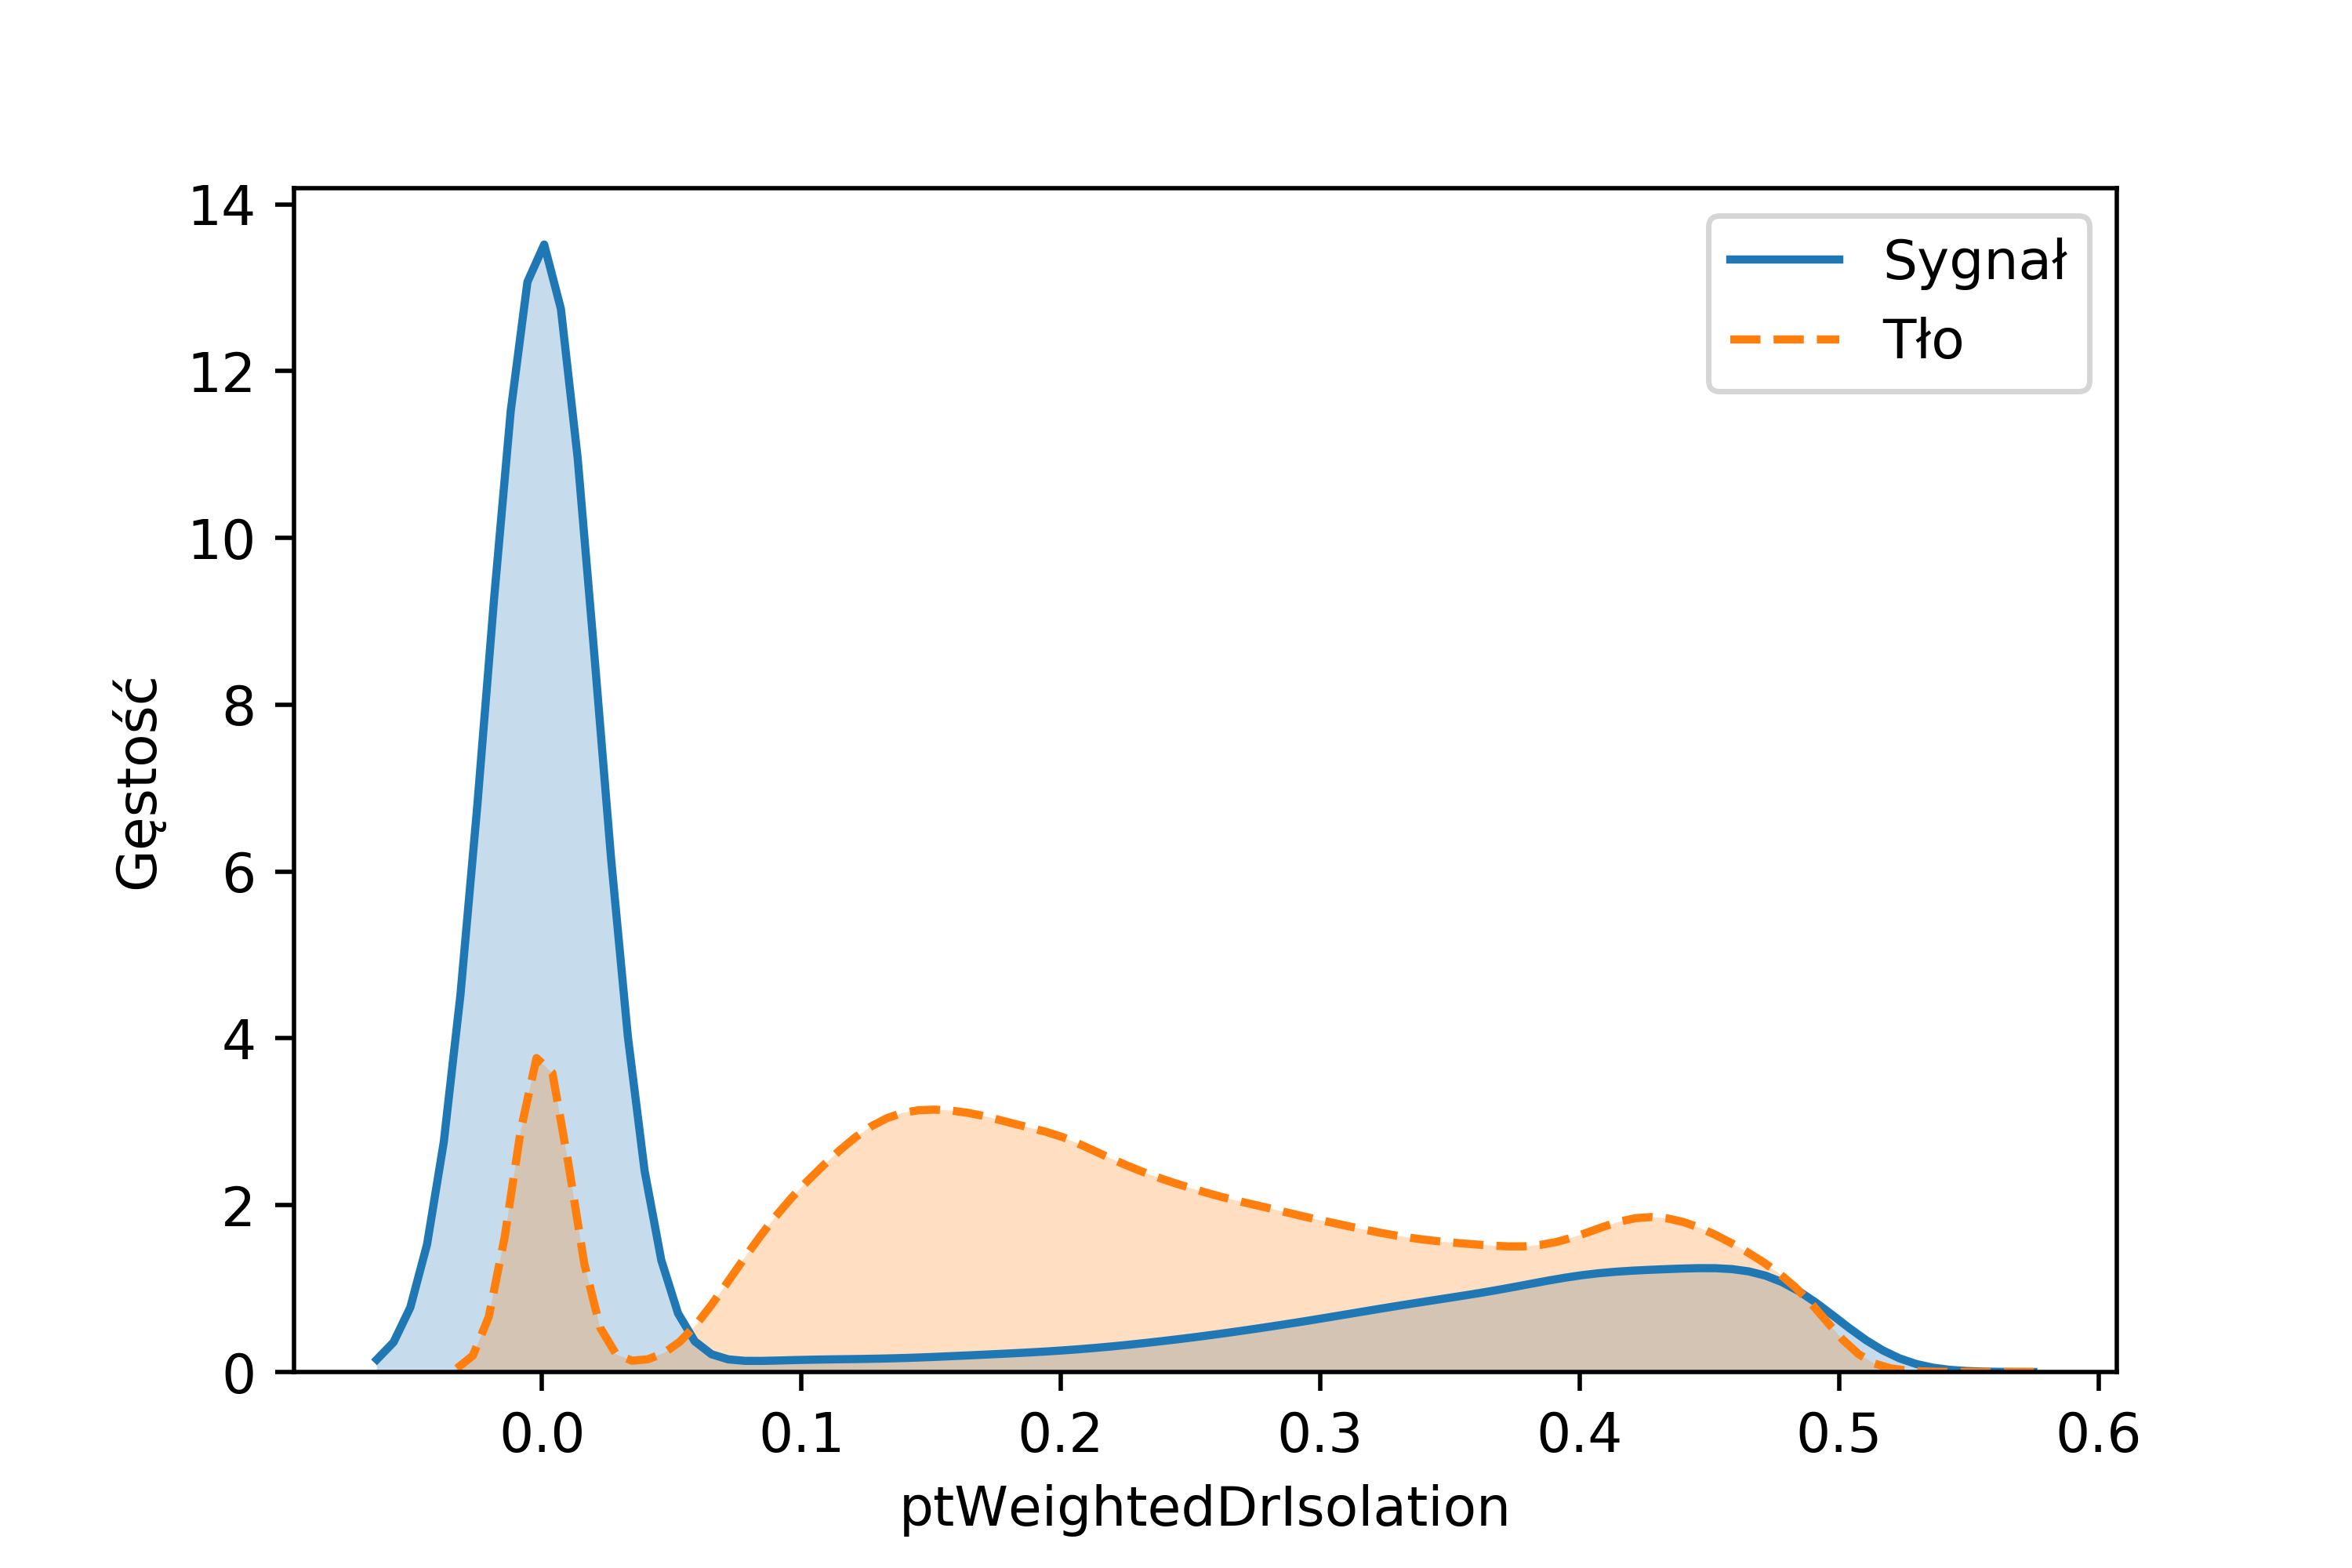
\includegraphics[width=0.7\textwidth]{difference.png}
	\caption{Różnice w rozkładzie przykładowej zmiennej dla sygnału i tła}
	\label{fig:diff}
	\end{figure}
		
	Niestety można zauważyć również różnice między danymi symulacyjnymi a danymi eksperymentalnymi w rozkładach zmiennych objaśniających, także nie ma pewności, że model dający dobre wyniki na danych symulacyjnych będzie dawał równie dobre wyniki na danych eksperymentalnych.		
		
    \chapter{Metodologia (architektura?) TODO}
	Aby dokonywać klasyfikacji sygnału zastosowano różne modele predykcyjne opierające się na metodach opisanych w rozdziale \ref{ch:wstep}.
	\section{Model oparty o same klasyfikatory}
	\label{sec:mod1}
	Prosty model, składający się z jednego neuronu, który przyjmuje jako zmienne objaśniające odpowiedzi wcześniej używanych klasfikatorów (patrz rozdział \ref{ch:dane}). Jest to średnia ważona odpowiedzi klasyfikatorów na którą nałożona jest funkcja sigmoid. Wielkość batcha została ustalona na 128, do optymalizacji został użyty algorytm \textit{Adam} ze stałą uczenia $\gamma = 10^{-3}$. Model uczony był przez cztery epoki (cztery razy przetwarzał każdą obserwację).
	\section{Sieć neuronowa TODO: zmienić nazwę}
	\label{sec:mod2}
	Kolejny model był oparty o wszystkie dane, jego architekturę przedstawiono na rysunku \ref{fig:nn1}. Składa się z sześciu warstw gęstych, o wielkości 32 neuronów każda. Jako funkcje aktywacji zastosowano funkcje ReLU. Inne parametry zostały ustalone tak samo jak dla modelu w sekcji \ref{sec:mod1}. Ten model zwany jest później \textit{Stara sieć}.
	\begin{figure}
	\centering
	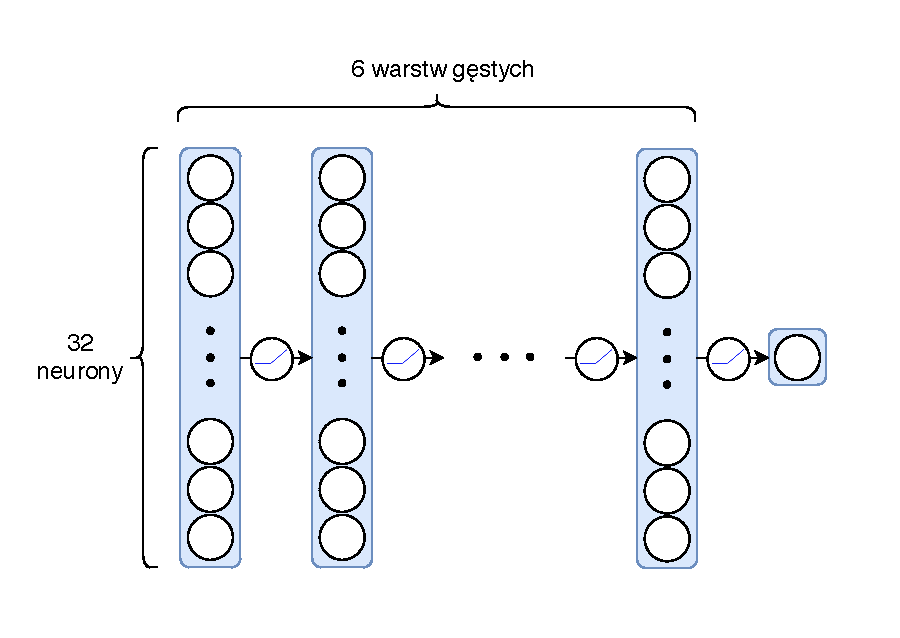
\includegraphics[width=0.8\textwidth]{neural_net.pdf}
	\caption{TODO}
	\label{fig:nn1}
	\end{figure}
	
	\section{Poprawiona sieć neuronowa TODO: zmienić nazwę}
	Na postawie optymalizacji hiperparametrów przy pomocy losowego przeszukiwania został wybrany najlepszy model oparty o gęste sieci neuronowe. Optymalizowano parametry takie jak: wielkość batcha, stała uczenia, wielkość i liczba warstw ukrytych, funkcja aktywacji, liczba epok, występowanie warstwy \textit{batch normalization} i występowanie callbacka %TODO nazwa
	. Otrzymana architektura znajduje się na rysunku \ref{fig:nn2}. 
	
	Wybrany model ma dwie warstwy gęste po 256 neuronów każda, zatem widać że model jest płytszy i szerszy niż opisany w sekcji \ref{sec:mod2}. Jako funkcja aktywacji jest tutaj użyty sigmoid, a dodatkowo zastosowana jest warstwa \textit{batch normalization}. Użyta wielkość batcha to 256, do optymalizacji  zastosowano algorytm \textit{Adam} ze stałą uczenia $\gamma = 5\cdot 10^{-4}$ oraz callbackiem %TODO nazwa
	zmniejszającym stałą uczenia $\gamma$ na wypłaszczeniu %TODO czego? 
	przez czynnik 0.2 do minimalnej wartości $\gamma = 10^{-5}$. Moodel był uczony przez sześć epok. Ten model zwany jest później \textit{Nowa sieć}.
	\begin{figure}
	\centering
	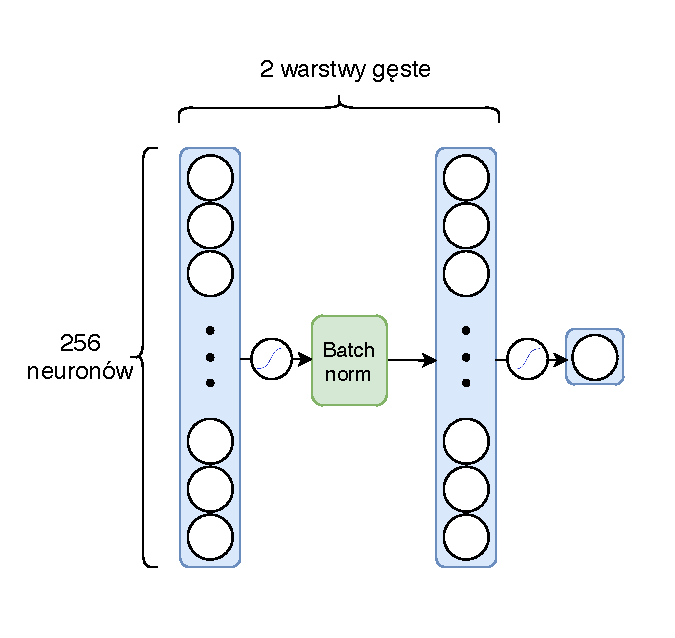
\includegraphics[width=0.7\textwidth]{best_neural_net.pdf}
	\caption{TODO}
	\label{fig:nn2}
	\end{figure}	
	
	\section{XGBoost}
	Model oparty na XGBoost składał się ze 100 drzew decyzyjnych o maksymalnej głębokości 3. %TODO coś więcej
	\begin{figure}
	\centering
	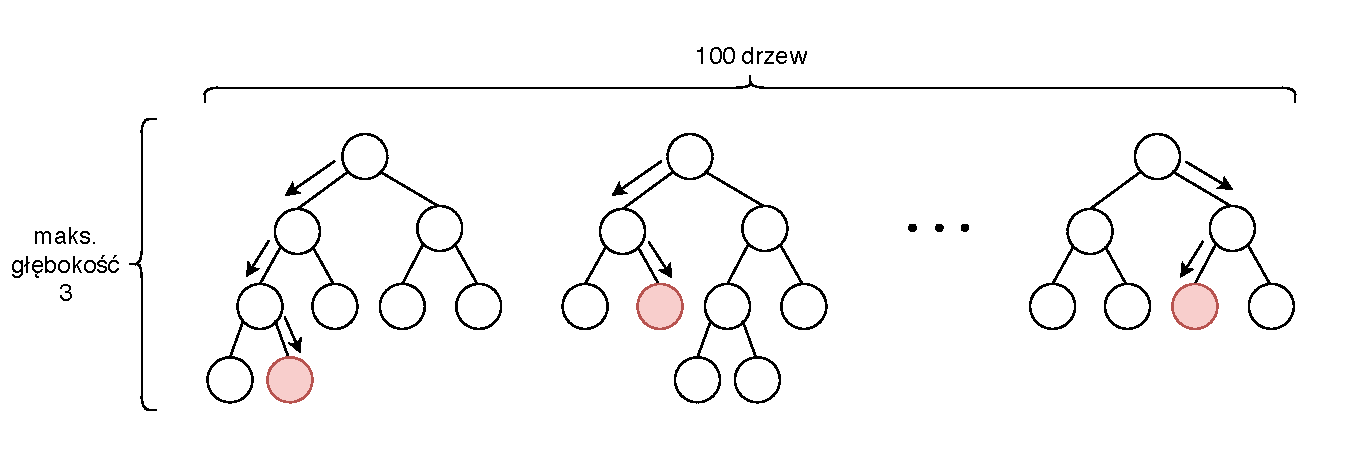
\includegraphics[width=1.0\textwidth]{xgb.pdf}
	\caption{TODO}
	\label{fig:xgb}
	\end{figure}
    
    \chapter{Wyniki}
	Modele były najpierw uczone na wszystkich zmiennych objaśniających oraz na danych z pominięciem odpowiedzi klasyfikatorów. Dzięki temu można porównać wyniki z wcześniej używanymi modelami. Po dokonaniu analizy istotności zmiennych zauważono, że istnieje jedna zmienna (leg\_2\_byCombinedIsolationDeltaBetaCorrRaw3Hits, patrz rozdział \ref{ch:dane}), która jest najbardziej istotna dla wszystkich modeli. Jako, że zmienna ta różni się na danych symulacyjnych oraz eksperymentalnych, postanowiono wytrenować również modele bez tej zmiennej.
    
	W tabeli \ref{tab:wyniki} znajdują się wyniki ROC AUC otrzymane dla wszystkich modeli. Modele (poza modelem opisanym w sekcji \ref{sec:mod1}) uczone były w trzech trybach: na pełnych danych, na danych z wyłączeniem odpowiedzi klasyfikatorów oraz na pełnych danych z wyłączeniem najlepszej zmiennej. Dla porównania zamieszczono wynik najlepszego z wcześniejszych klasyfikatorów, którym okazał się leg\_2\_deepTau2017v1tauVSjet. 
	
	\begin{table}[H]
	\centering
	\begin{tabular}{lrrrrr}
	\toprule
	Tryb & Stara sieć & Nowa sieć & XGBoost & Same klas. & Najlepszy klas. \\
	\midrule
	Pełne dane & .9948 & .9979 & \textbf{.9985} & $-$ & $-$ \\
	Bez klas. & .9940 & .9949 & \textbf{.9956} & $-$ & .9945 \\
	Bez najlepszej & .9977 & .9972 & \textbf{.9985} & $-$ & $-$ \\
	Same klas. & $-$ & $-$ & $-$ & .9956 & $-$  \\
	\bottomrule
	\end{tabular}
	\caption{Wartość ROC AUC dla wszystkich modeli na zbiorze testowym, pogrubioną czcionką zaznaczono najlepszy wynik.}
	\label{tab:wyniki}
	\end{table}
	
	Na rysunkach \ref{fig:res_best}, \ref{fig:res_new} i \ref{fig:res_disc} przedstawiono fragmenty krzywych ROC dla wybranych modeli. Na wykresach osie są zamienione, więc lepszy model ma mniejsze pole pod krzywą. Zakres TPR na wykresach został zmniejszony aby lepiej uwidocznić różnice między modelami.
	
	\begin{figure}
	\centering
	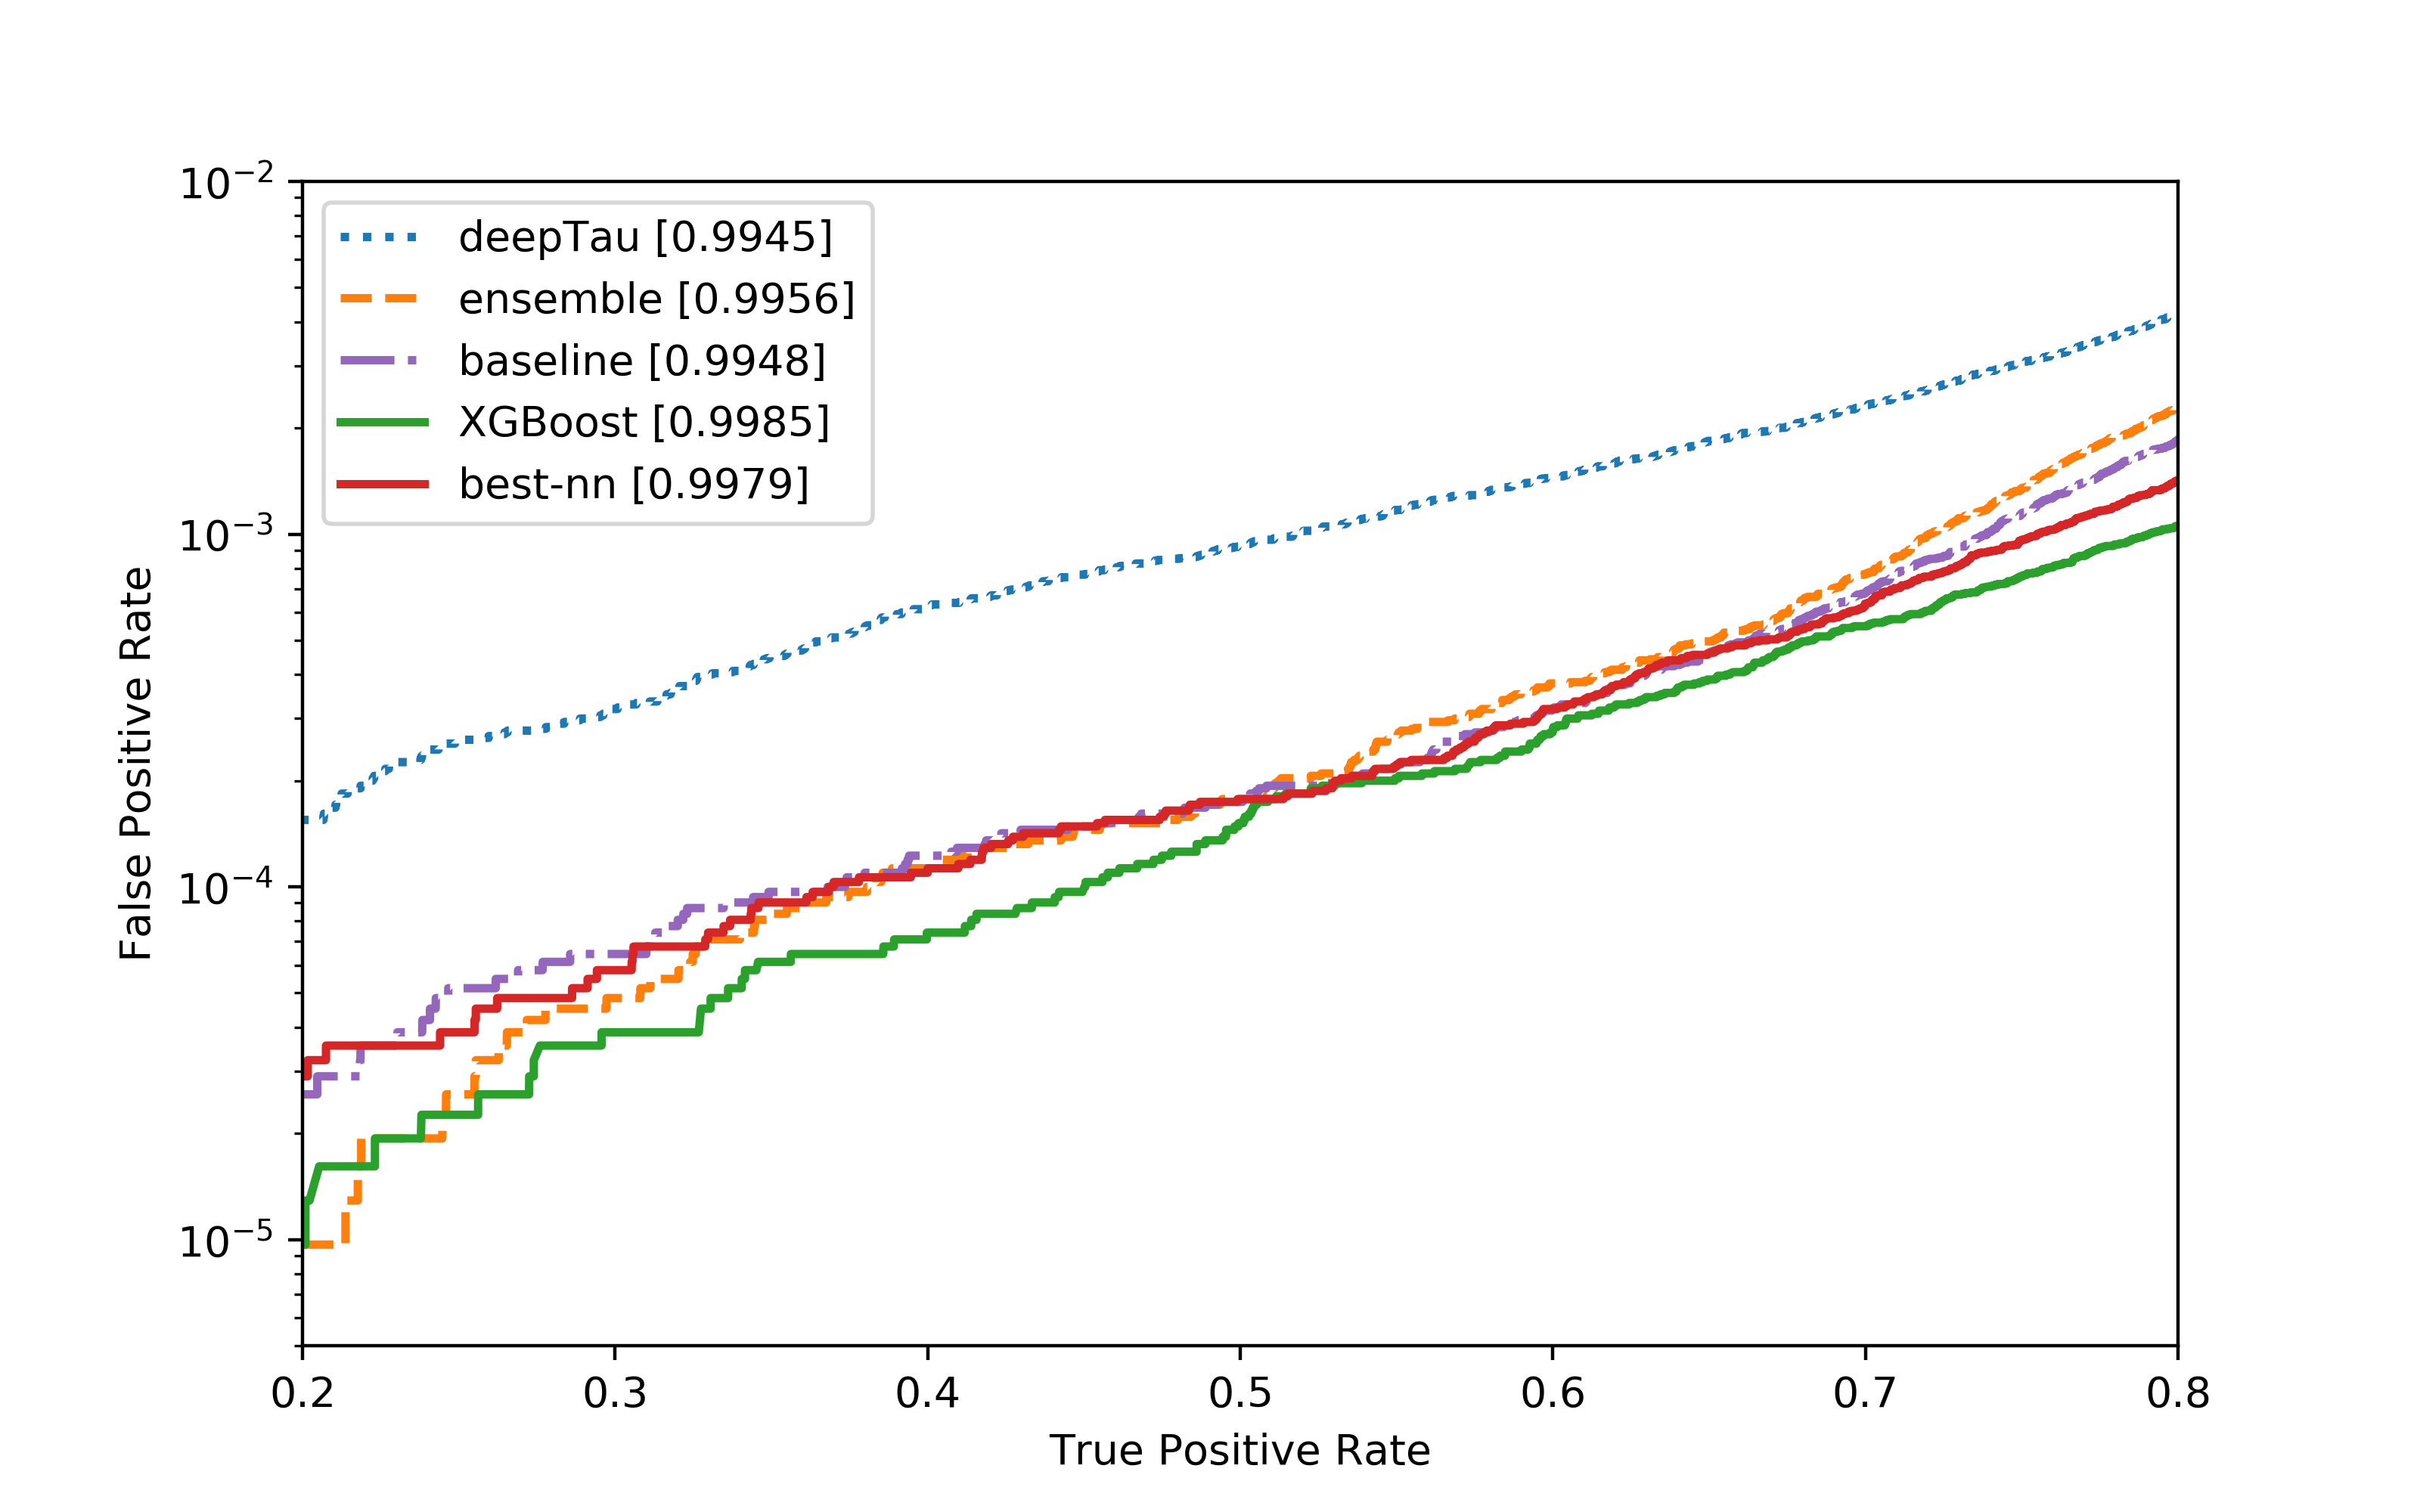
\includegraphics[width=1.\textwidth]{best_models.png}
	\caption{Porówanie najlepszych modeli. Stara sieć, nowa sieć oraz XGBoost były uczone na pełnych danych, deepTau na danych bez klasyfikatorów.}
	\label{fig:res_best}
	\end{figure}  
	
	\begin{figure}
	\centering
	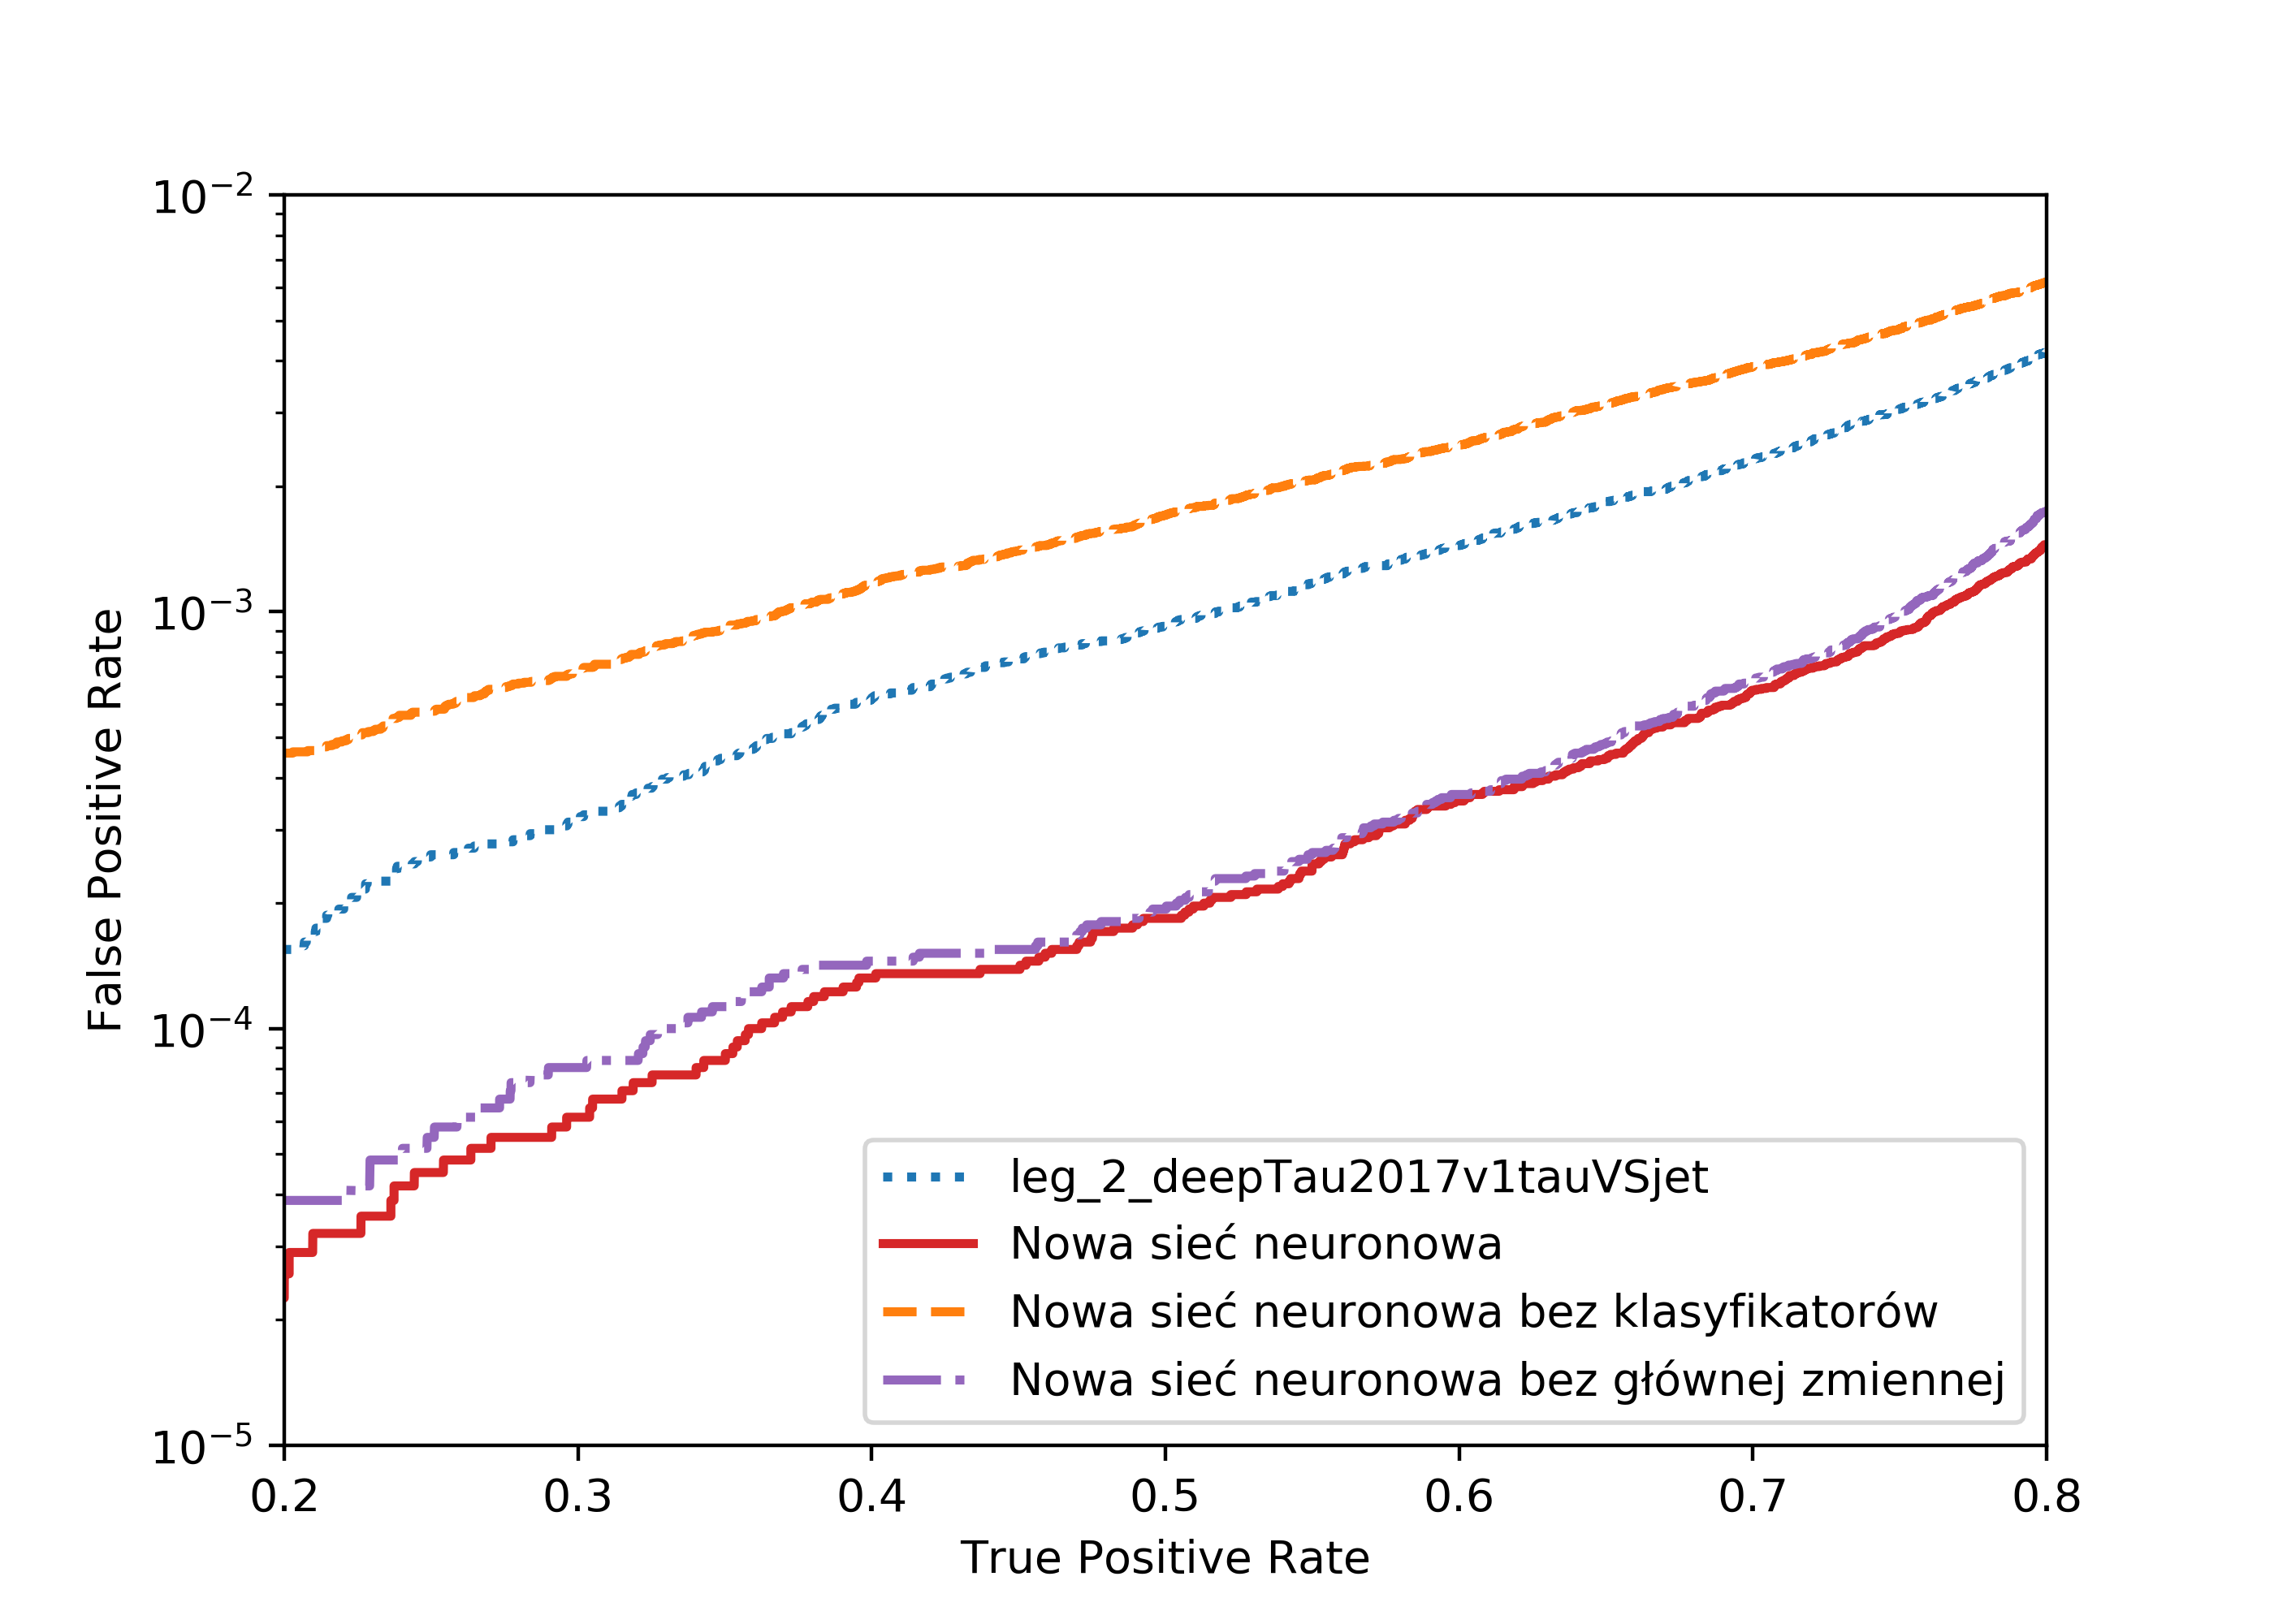
\includegraphics[width=1.\textwidth]{new_network.png}
	\caption{Porównanie wszystkich trybów uczenia nowej sieci z najlepszym klasyfikatorem.}
	\label{fig:res_new}
	\end{figure} 	
	
	\begin{figure}
	\centering
	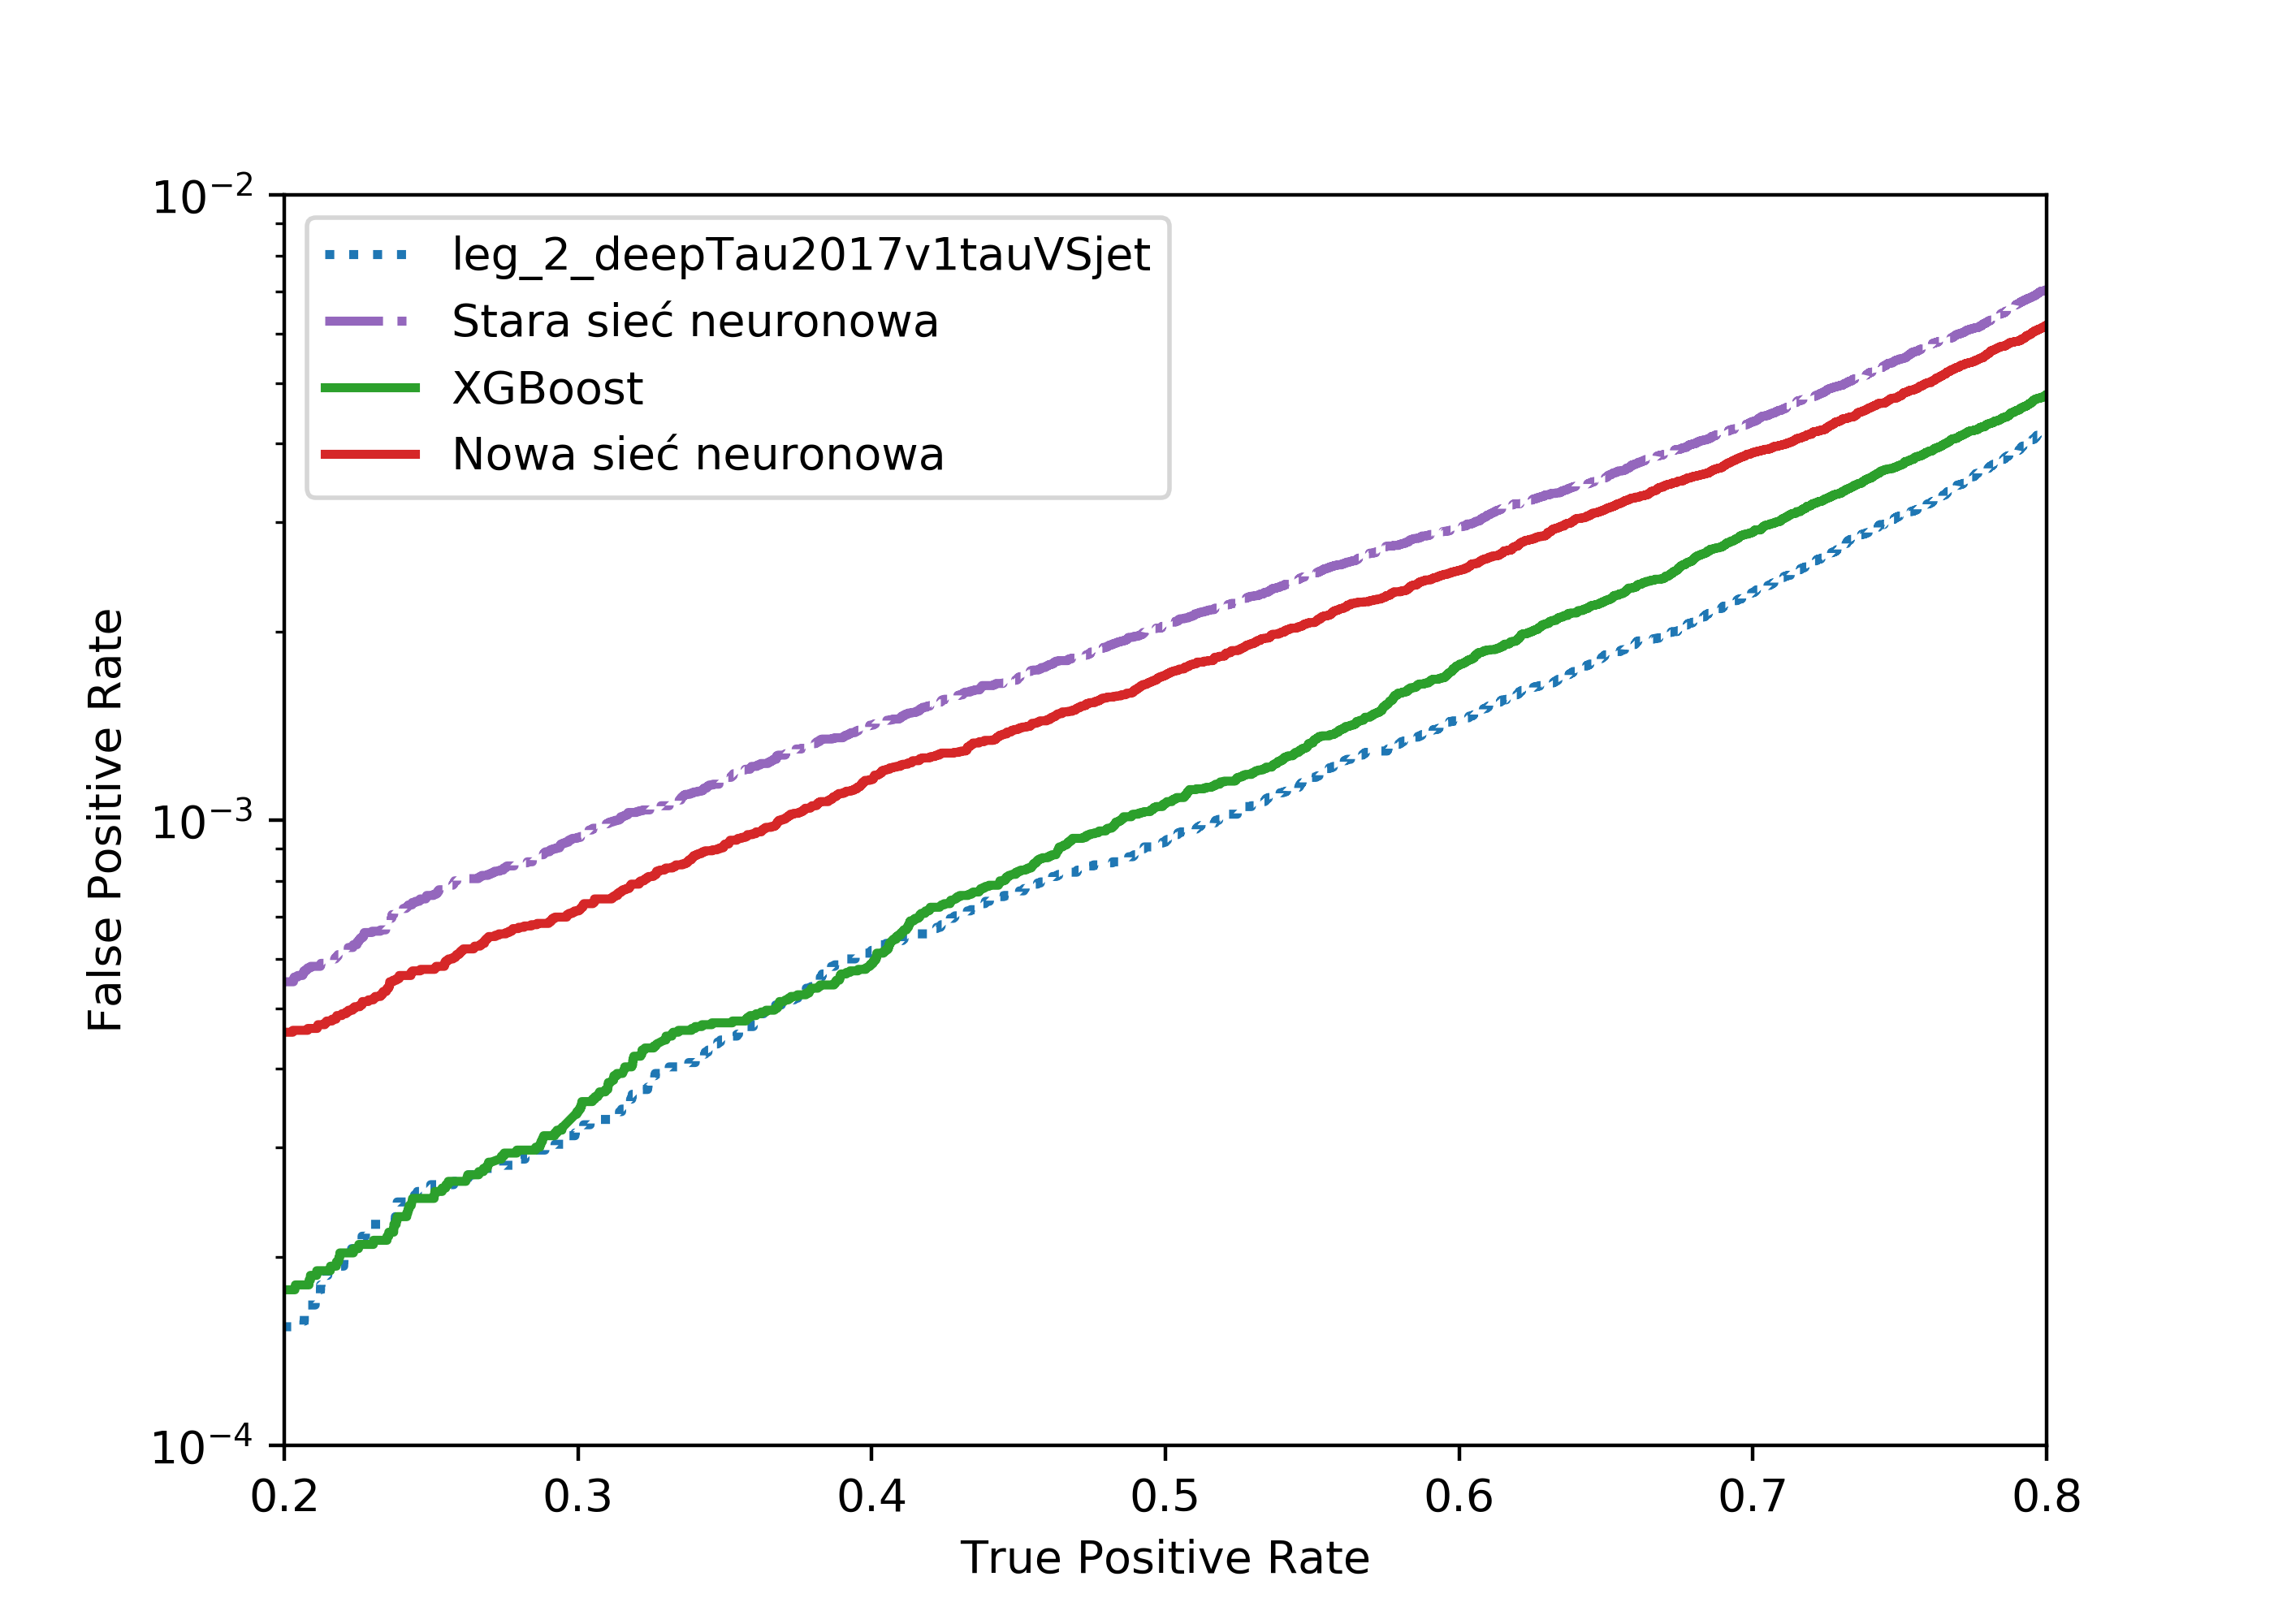
\includegraphics[width=1.\textwidth]{without_disc.png}
	\caption{Porównanie modeli uczonych na danych bez klasyfikatorów.}
	\label{fig:res_disc}
	\end{figure} 
	
    %TODO wyniki na eksperymentalnych?
    %TODO wyniki na mieszaninach?
    
    \chapter{Dyskusja}
    \chapter{Podsumowanie}
    
    \addcontentsline{toc}{chapter}{Bibliografia}
    \printbibliography
    
\end{document}
